\documentclass[12pt] {article}

%%% Preambuła %%%
\usepackage[T1]{fontenc}
\usepackage[polish]{babel}
\usepackage[utf8]{inputenc}
\usepackage{lmodern}
\usepackage[hidelinks]{hyperref}
\usepackage{mathptmx}
\usepackage{float}
\usepackage{graphicx}
\usepackage{amsmath}
\usepackage{xcolor}
\usepackage{listings}
\usepackage{geometry}
\usepackage{tocloft}
\usepackage{subcaption}
\usepackage{indentfirst}
\selectlanguage{polish}

\lstset{basicstyle=\ttfamily,
  showstringspaces=false,
  commentstyle=\color{red},
  keywordstyle=\color{blue},
  basicstyle=\ttfamily\footnotesize,
  columns=fullflexible,
  breaklines=true
}

\renewenvironment{abstract}
 {\small
  \begin{center}
  \bfseries \abstractname\vspace{-.5em}\vspace{0pt}
  \end{center}
  \list{}{%
    \setlength{\leftmargin}{5mm}% <---------- CHANGE HERE
    \setlength{\rightmargin}{\leftmargin}%
  }%
  \item\relax}
 {\endlist}

\renewcommand{\cftsecleader}{\cftdotfill{\cftdotsep}} 
\geometry{a4paper, total={170mm,257mm}, left=20mm, top=20mm,}

%%% Strona tytułowa %%%
\title {
	\large Automaty komórkowe \\
    \normalsize Projekt 1: rozszerzony automat Life
    }

\author {Arkadiusz Kasprzak}
\date{}
	
\begin{document}


%%% Strona tytułowa %%%
\maketitle

%%% Streszczenie %%%
\begin{abstract}
Niniejszy dokument stanowi sprawozdanie z pierwszego projektu realizowanego w ramach przedmiotu \textit{Automaty komórkowe}. Tematem projektu było opracowanie interaktywnej aplikacji internetowej implementującej automat 2D (tzw. \textit{Life-like}) na siatce kwadratowej z periodycznymi warunkami brzegowymi i otoczeniem Moore'a. W sprawozdaniu omówione zostaną podstawowe zagadnienia teoretyczne opisujące implementowany automat, podstawy implementacji oraz testy działania - w tym zaobserwowane charakterystyczne struktury. 
\end{abstract}

%%% Spis treści %%%
\tableofcontents

\newpage 

\section{Wstęp}
Celem projektu było stworzenie aplikacji implementującej dwuwymiarowy automat komórkowy stanowiący rozszerzenie popularnego automatu \textit{Life}. W swojej podstawowej postaci automat ten jest zdefiniowany na dwuwymiarowej sieci kwadratowej, gdzie każda z komórek może znajdować się w jednym z dwóch stanów (żywa/martwa) \cite{malarz}. Automat ten opiera się na regule 23/3 (jeśli w otoczeniu żywej komórki są 2 lub 3 inne żywe komórki, to pozostaje ona żywa oraz jeśli w otoczeniu martwej komórki znajdują się 3 komórki żywe, to komórka ta staje się żywa). Zarówno w klasycznym automacie \textit{Life}, jak i w prezentowanej w ramach projektu wersji stosuje się otoczenie Moore'a (czyli obejmujące komórki mające z komórką aktualnie przetwarzaną wspólne zarówno krawędzie, jak i wierzchołki). Implementowana w ramach projektu wersja automatu pozwala na stosowanie reguł innych niż 23/3 (dlatego stanowi rozszerzenie oryginalnego automatu - ang. \textit{Life-like}). Projekt stosuje periodyczne warunki brzegowe (sieć nie jest więc, w przeciwieństwie do automatu oryginalnego, nieskończona).



\section{Implementacja i opis interfejsu}
Projekt zaimplementowany został w formie prostej strony internetowej (klient) z użyciem technologii HTML5, CSS3 oraz języka JavaScript. Wizualizacja działania automatu oparta została o animację wykonaną za pomocą elementu \lstinline{<canvas>}. W celu szybkiego przygotowania strony wykorzystana została biblioteka Bootstrap. Wykres gęstości wykonany został natomiast z pomocą biblioteki D3 (Data-Driven Documents). Projekt nie wymaga instalowania lub pobierania żadnych dodatkowych zależności - wszystkie potrzebne pliki bibliotek zawarte zostały w katalogu \lstinline{resources}. 


Projekt korzysta z funkcjonalności wprowadzonych w standardzie ECMAScript 6 - do jego działania może więc być konieczna stosunkowo nowa wersja przeglądarki. Projekt został przetestowany na przeglądarkach: Google Chrome (wersja 80.0.3987.132) oraz Firefox (wersja 73.0.1). 

\begin{figure}[H]
\centering
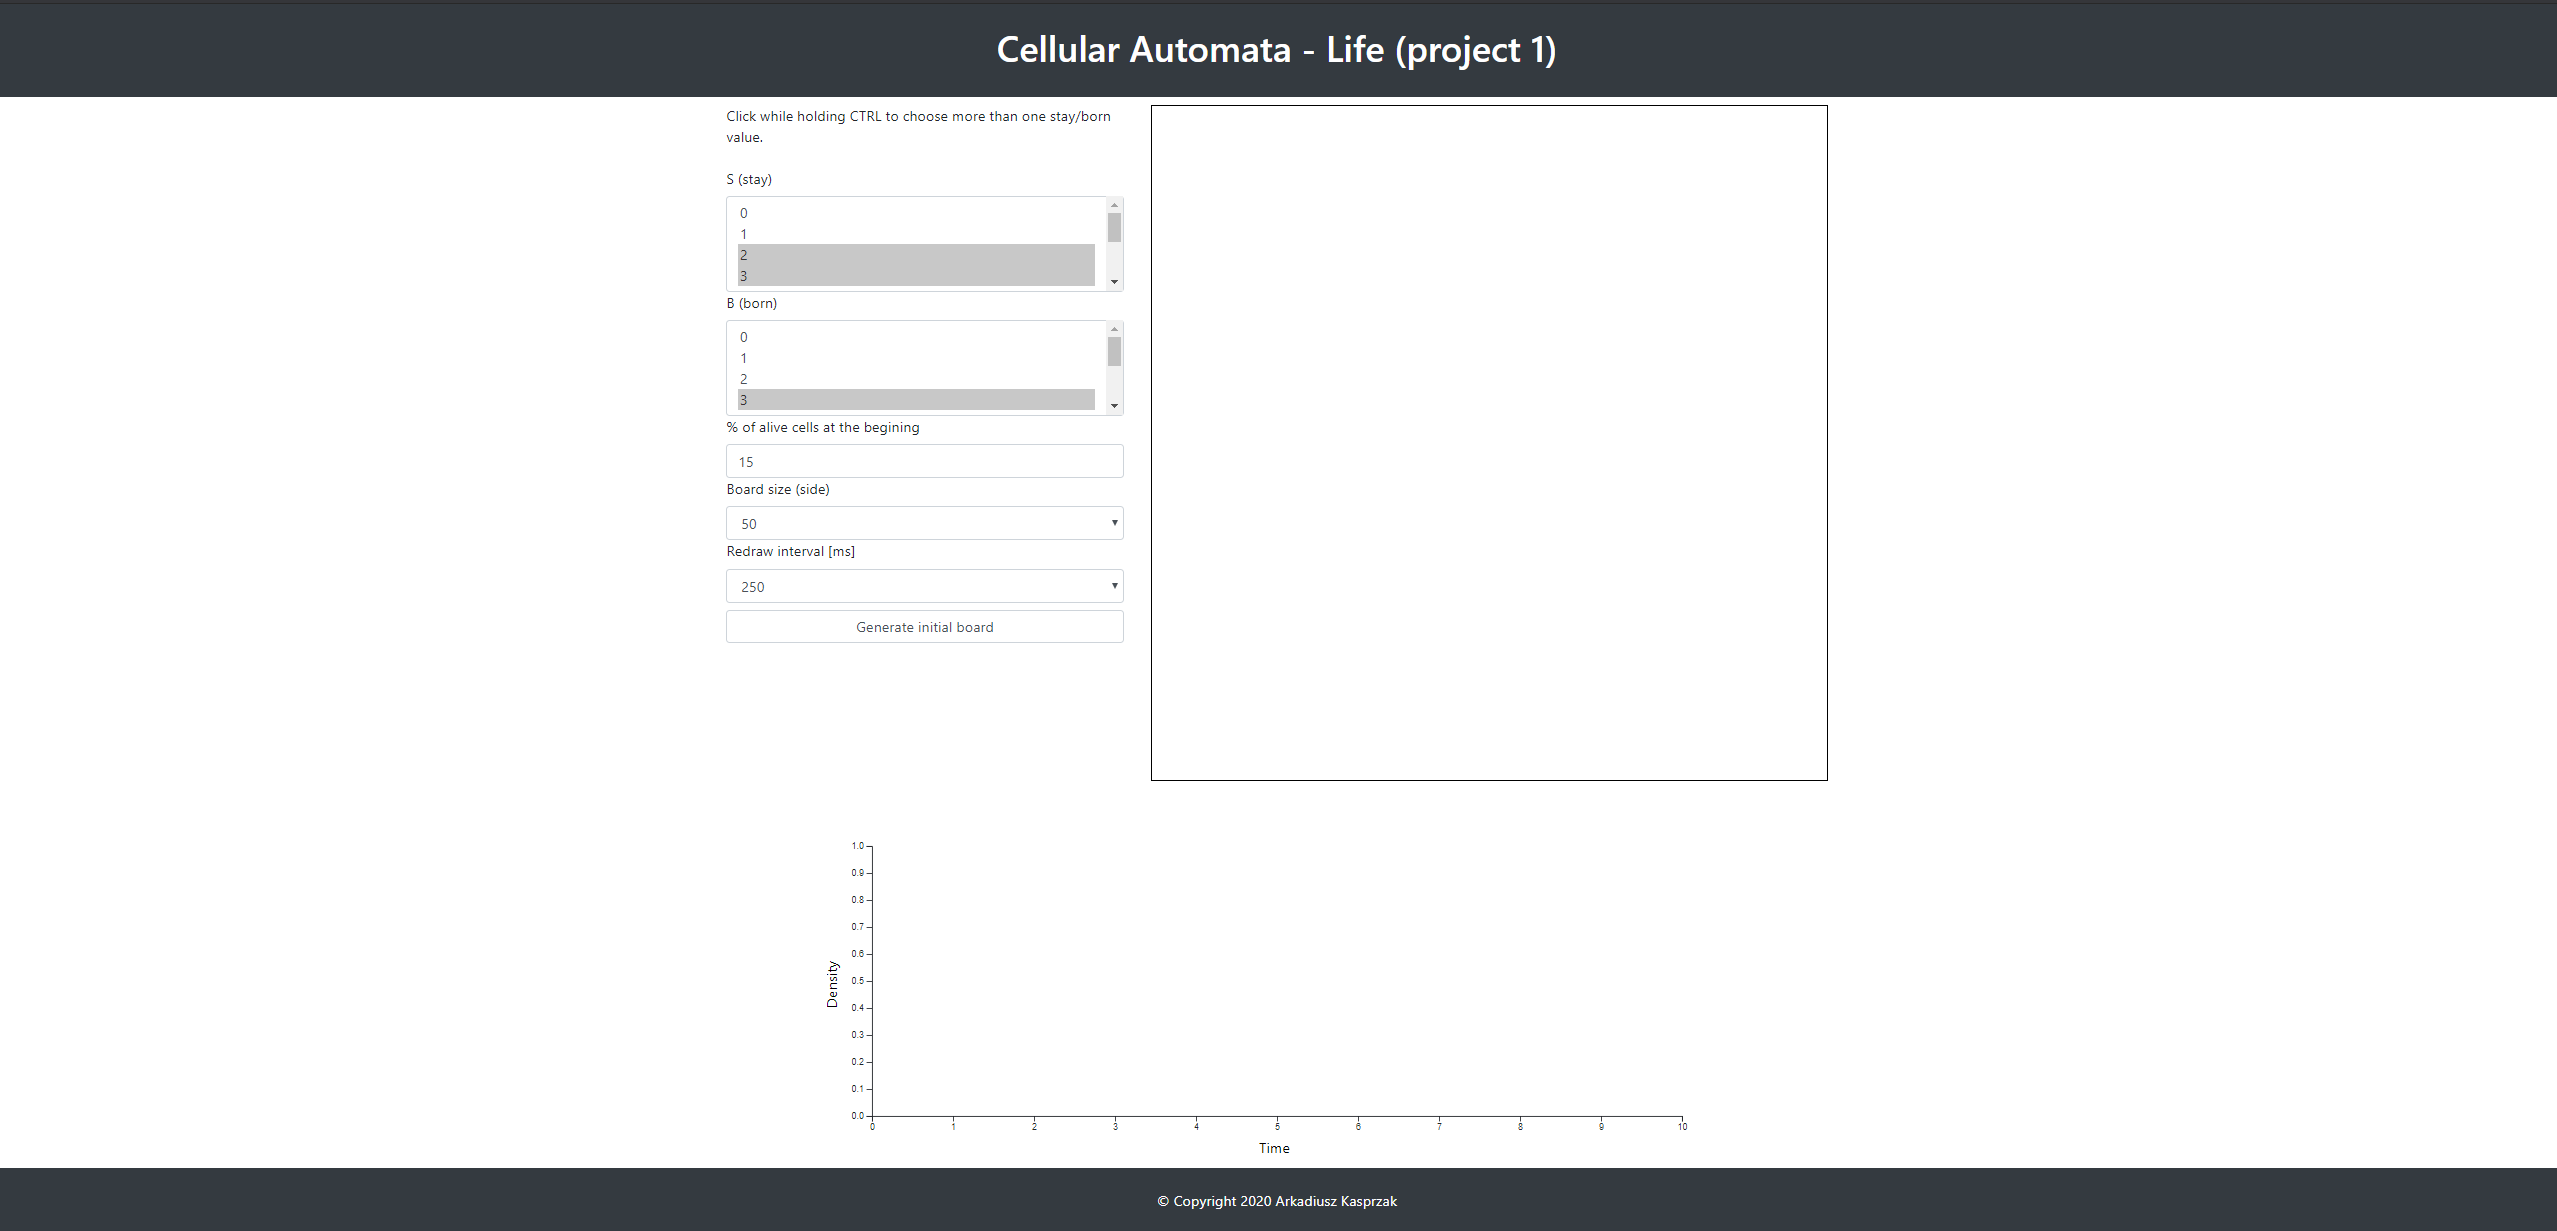
\includegraphics[width=\textwidth]{res/interface1.png}
\caption{Interfejs przygotowanej aplikacji zaraz po uruchomieniu. Po lewej widoczne menu konfiguracji automatu, po prawej prostokąt na którym wyświetlana będzie symulacja, w dolnej części natomiast wykres gęstości żywych komórek.}
\label{fig:rys1}
\end{figure} 
\newpage

Rysunek \ref{fig:rys1} stanowi zrzut ekranu przedstawiający aplikację w stanie zaraz po uruchomieniu. Widoczne na nim są trzy podstawowe elementy aplikacji - menu pozwalające na konfigurację działania automatu widoczne - po lewej, prostokąt, w którym wyświetlana będzie animacja - po prawej oraz wykres gęstości żywych komórek w dziedzinie czasu. Użytkownik ma możliwość wyboru reguł (\textit{stay/born}) działania automatu, początkowej gęstości żywych komórek, rozmiaru siatki, na której prowadzona jest symulacja oraz szybkości działania symulacji. 


Wybór odpowiedniej konfiguracji przenosi użytkownika do kolejnego ekranu, gdzie możliwe jest wygenerowanie odpowiednich warunków początkowych (poprzez kilkukrotne powtarzanie operacji losowania lub manualną zmianę stanu każdej z komórek poprzez jej naciśnięcie). Po zakończeniu tej czynności użytkownik może rozpocząć symulację. Działającą symulację można w dowolnym momencie zatrzymać a następnie wznowić (rys. \ref{fig:rys2}).

\begin{figure}[H]
\centering
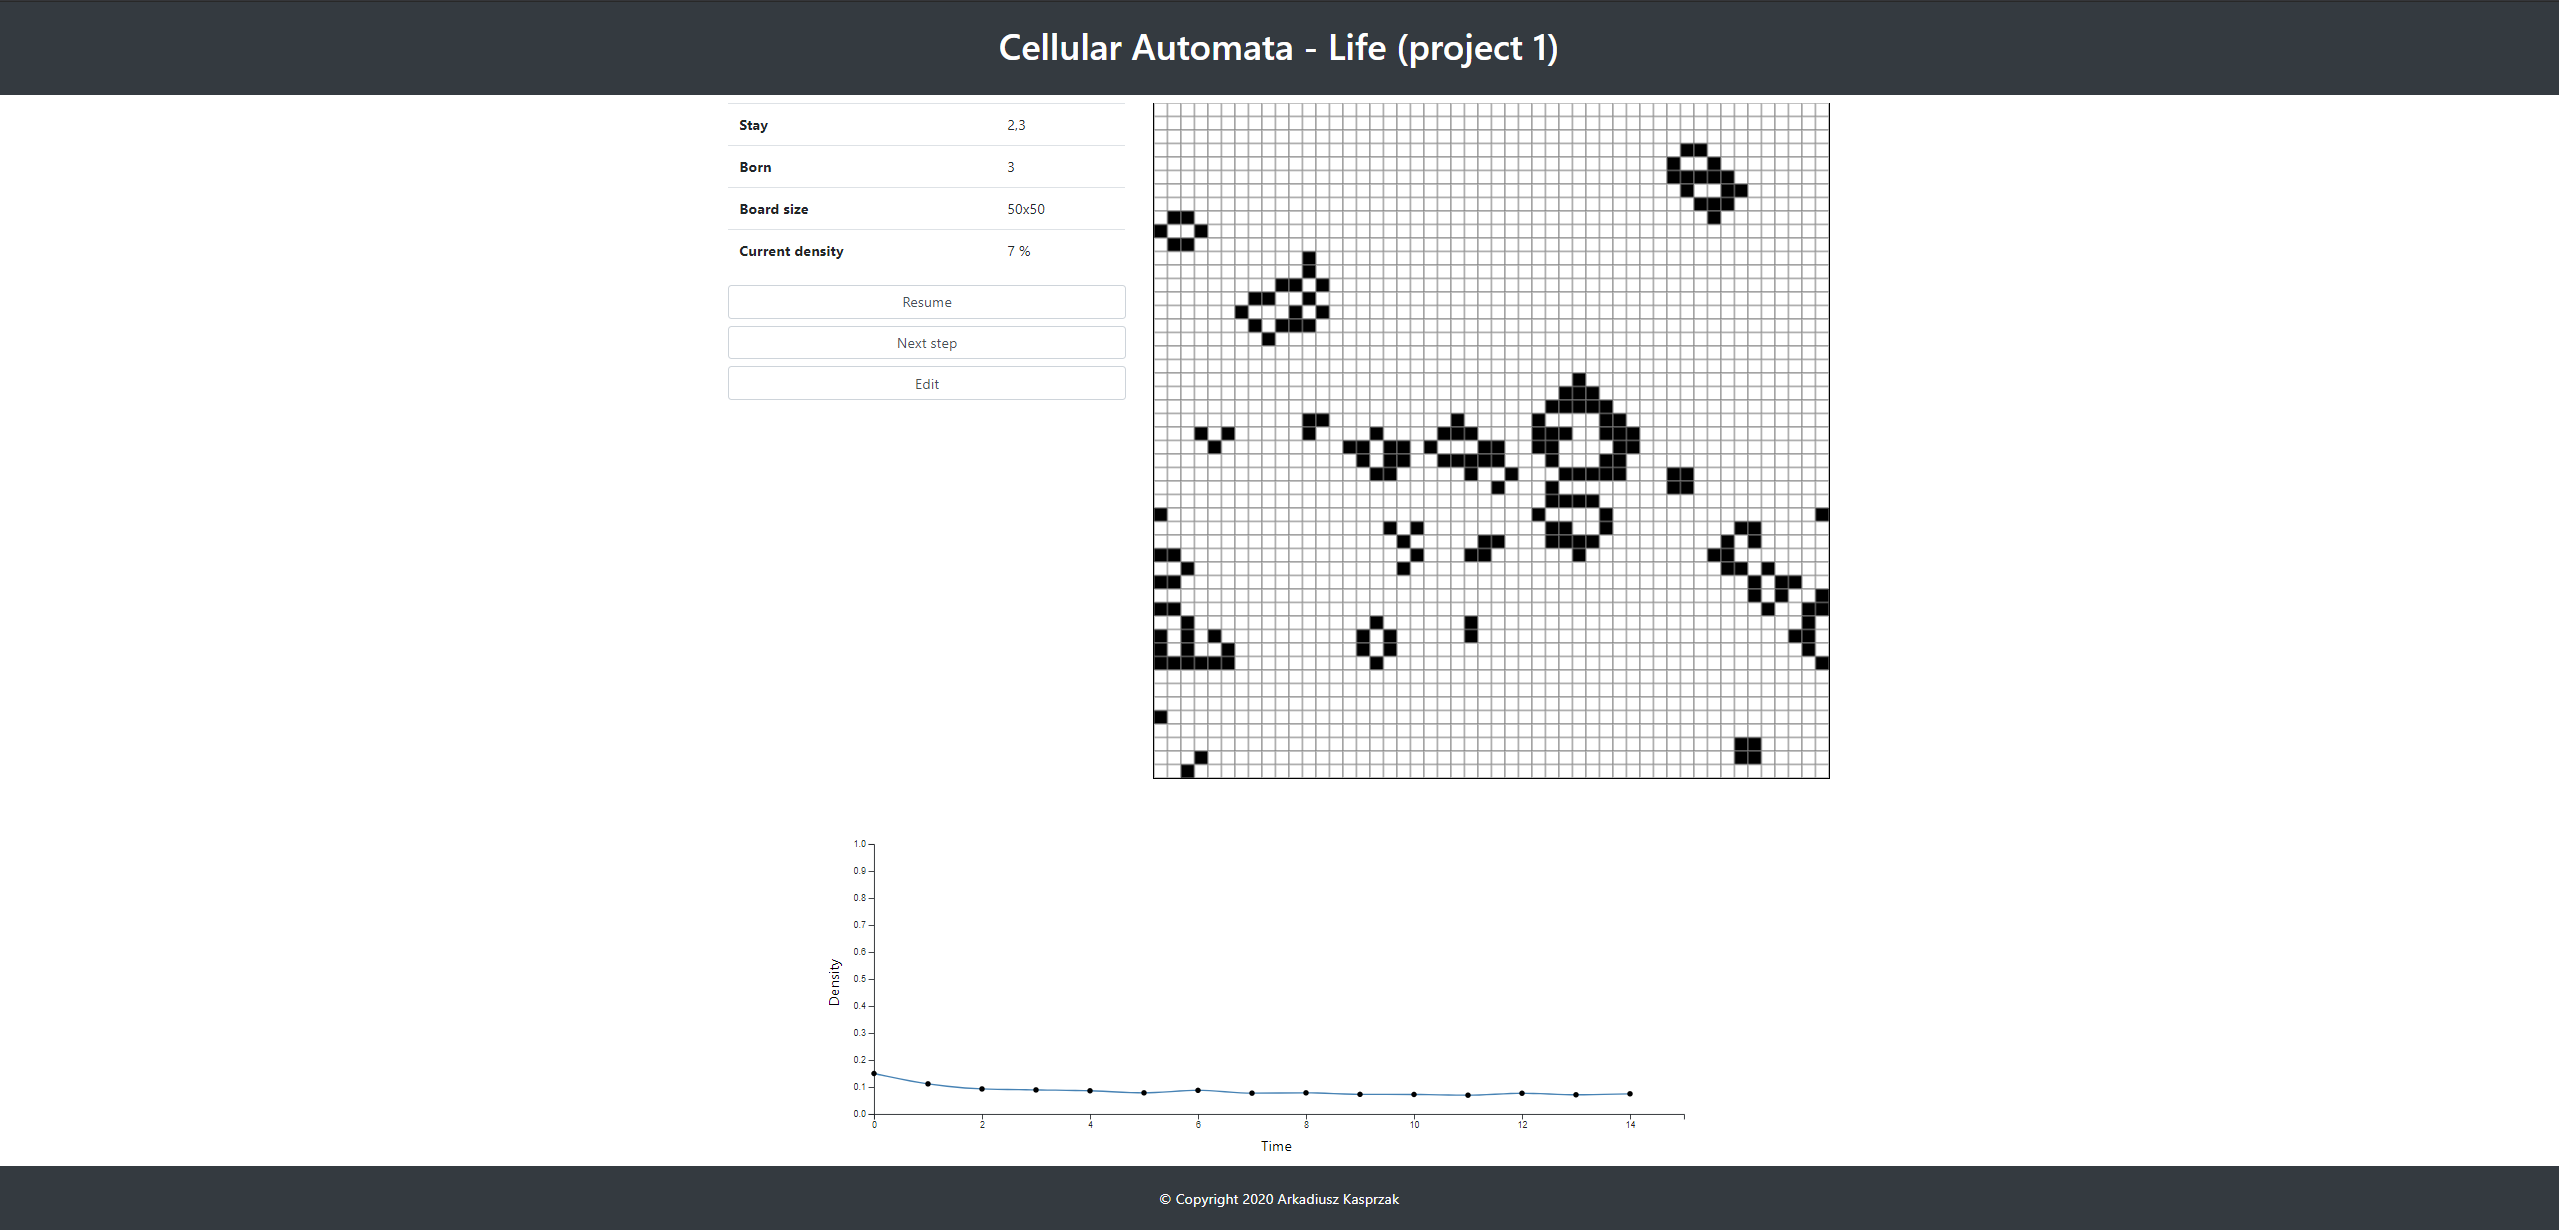
\includegraphics[width=\textwidth]{res/interface2.png}
\caption{Interfejs przygotowanej aplikacji po zatrzymaniu działania symulacji. Widoczne możliwe opcje wznowienia symulacji, wykonania pojedynczego jej kroku oraz powrotu do konfiguracji.}
\label{fig:rys2}
\end{figure}


\section{Testy działania}
Dowolność w specyfikacji reguły początkowej pozwala na zaobserwowanie wielu interesujących przypadków działania automatu. Domyślnie testy przeprowadzane były na sieci o rozmiarze $50\times50$ (z wyjątkiem kilku sytuacji, w których inny rozmiar zostanie wyszczególniony w sprawozdaniu). Niniejsze sprawozdanie zawiera opis jedynie kilku wybranych testów przeprowadzonych przez autora - ilość interesujących struktur możliwych do uzyskania za pomocą stworzonego programu jest znacznie większa.


Testy rozpoczęte zostały od klasycznej reguły \textbf{23/3}. Wygenerowana została początkowa plansza o gęstości $0.6$. Przebieg symulacji zaobserwować można na rysunku \ref{fig:life123}. Przedstawiony tam został stan symulacji w chwili początkowej - widoczna znaczna gęstość żywych komórek, po około 470 krokach oraz po osiągnięciu stanu stabilnego - po około 650 krokach. Bardzo charakterystyczny jest fakt. iż już w pierwszym kroku symulacji stosunkowo znaczna gęstość 0.6 zredukowana została do około 0.15. Na rysunku \ref{fig:life2} zaobserwować można niektóre ze struktur charakterystycznych dla automatu \textit{Life} - blok (oznaczony kolorem czerwonym), kryształ (nazywany też ulem - oznaczony kolorem zielonym) oraz łódź (kolor niebieski). Cechą charakterystyczną tego typu struktur jest ich stabilność (bez zewnętrznej ingerencji pozostają identyczne niezależnie od kroku czasowego). 

\begin{figure}[H]
    \begin{minipage}[t]{.3\textwidth}
        \centering
        
\includegraphics[width=\textwidth]{res/23_3_first.png}
        \subcaption{Krok 0}\label{fig:life1}
    \end{minipage}
    \hfill
    \begin{minipage}[t]{.3\textwidth}
        \centering
        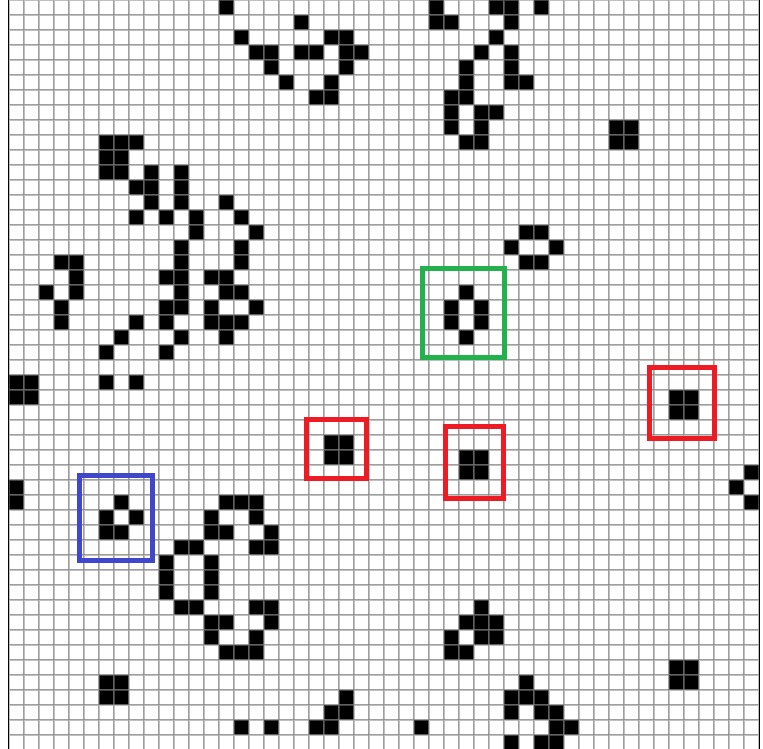
\includegraphics[width=\textwidth]{res/23_3_470.png}
        \subcaption{Krok 470}\label{fig:life2}
    \end{minipage}
    \hfill
    \begin{minipage}[t]{.3\textwidth}
        \centering
        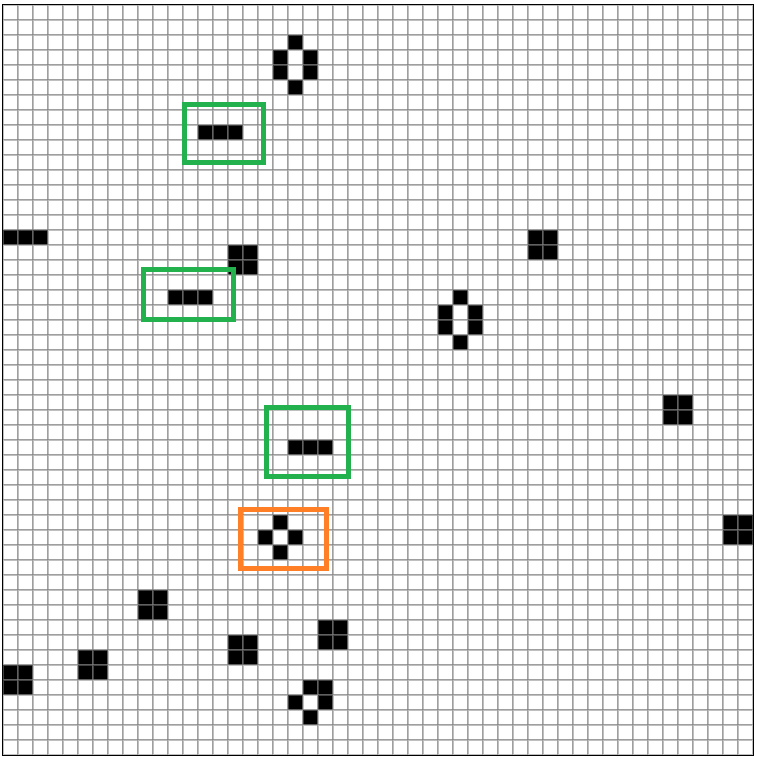
\includegraphics[width=\textwidth]{res/23_3_650.png}
        \subcaption{Krok 650}\label{fig:life3}
    \end{minipage}  
    \caption{Przebieg działania automatu dla reguły 23/3 w trzech wybranych chwilach czasowych.}
    \label{fig:life123}
\end{figure}


Na rysunku \ref{fig:life3}, przedstawiającym sytuację po ustabilizowaniu się automatu, poza wcześniej wymienionymi zaobserwować można jeszcze dwie inne interesujące struktury: stabilną strukturę koniczyny (kolor pomarańczowy) oraz najprostszy z tzw. oscylatorów - \textit{blinker} (oznaczony kolorem zielonym). Cechą charakterystyczną oscylatorów jest to, iż zmieniają swój stan w sposób okresowy. Rysunek \ref{fig:blinker} przedstawia proces ewolucji \textit{blinker'a}. 

\begin{figure}[H]
    \begin{minipage}[t]{.5\textwidth}
        \centering
        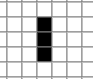
\includegraphics[width=0.5\textwidth]{res/b1.png}
        \subcaption{Pierwszy możliwy stan}\label{fig:b1}
    \end{minipage}
    \hfill
    \begin{minipage}[t]{.5\textwidth}
        \centering
        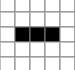
\includegraphics[width=0.5\textwidth]{res/b2.png}
        \subcaption{Drugi możliwy stan}\label{fig:b2}
    \end{minipage}
    \caption{Dwa możliwe stany \textit{blinker'a}. Struktura ta w każdym kroku czasowym zmienia swój stan na przeciwny.}
    \label{fig:blinker}
\end{figure}


Opisane struktury są oczywiście tylko niektórymi z możliwych do zaobserwowania podczas symulacji automatu z regułą 23/3. Podczas przeprowadzania innych symulacji pojawiło się ich znacznie więcej. Część z nich widoczna jest na rysunku \ref{fig:other}.

\begin{figure}[H]
    \begin{minipage}[t]{.3\textwidth}
        \centering
        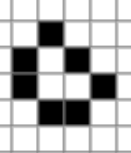
\includegraphics[width=0.6\textwidth]{res/bochenek.png}
        \subcaption{Bochenek - statyczny}\label{fig:o1}
    \end{minipage}
    \hfill
    \begin{minipage}[t]{.3\textwidth}
        \centering
        
\includegraphics[width=0.6\textwidth]{res/glider1.png}
        \subcaption{Szybowiec - początek lotu}\label{fig:o2}
    \end{minipage}
    \hfill
    \begin{minipage}[t]{.3\textwidth}
        \centering
        
\includegraphics[width=0.6\textwidth]{res/glider2.png}
        \subcaption{Szybowiec - po upływie kilku kroków czasowych}\label{fig:o3}
    \end{minipage}
    \caption{Pozostałe struktury zaobserwowane podczas wielokrotnych symulacji - statyczny bochenek oraz tzw. szybowiec (ang. \textit{glider}) - struktura okresowa poruszająca się po siatce (tutaj siatka $10\times10$).}
    \label{fig:other}
\end{figure}

\newpage

Kolejną testowaną regułą była reguła \textbf{1357/1357}. Charakteryzuje się ona pewną szczególną cechą - dowolny początkowy wzór jest, po pewnej liczbie kroków czasowych, powielany (stąd nazwa - replikator). Przykład działania widoczny na rysunku \ref{fig:rep}.


\begin{figure}[H]
    \begin{minipage}[t]{.3\textwidth}
        \centering
        
\includegraphics[width=\textwidth]{res/rep2.png}
        \subcaption{Krok 0}\label{fig:r4}
    \end{minipage}
    \hfill
    \begin{minipage}[t]{.3\textwidth}
        \centering
        
\includegraphics[width=\textwidth]{res/rep2_8.png}
        \subcaption{Krok 8}\label{fig:r5}
    \end{minipage}
    \hfill
    \begin{minipage}[t]{.3\textwidth}
        \centering
        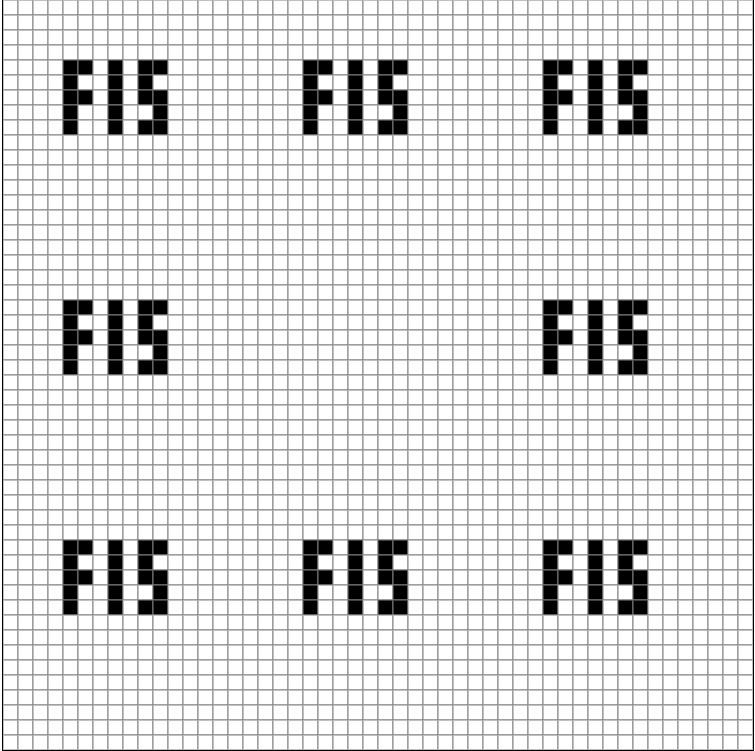
\includegraphics[width=\textwidth]{res/rep2_16.png}
        \subcaption{Krok 16}\label{fig:r6}
    \end{minipage}
    \caption{Przykład działania automatu o regule 1357/1357 - w ósmym kroku czasowym początkowy wzór jest powielany osiem razy.}
    \label{fig:rep}
\end{figure}

Testom poddana została również reguła \textbf{/2} - jest ona interesująca, ponieważ nie zawiera warunku pozwalającego żywym komórkom przeżyć przejścia do kolejnego kroku czasowego - tzn. wszystkie komórki żywe w kroku czasowym $t_n$ umierają przy przejściu do kroku $t_{n+1}$. Wynik przykładowej symulacji zawarty został na rysunku \ref{fig:seeds} - w tym wypadku, aby możliwe było dokładne zaobserwowanie działania automatu, symulacja przeprowadzona została na sieci o rozmiarze $100\times100$. Zaobserwować można znaczny wzrost gęstości żywych komórek - od wartości początkowej poniżej $0.01$ do stabilnej wartości około $0.2$. Jest to skutkiem niskiej wartości warunku na ożywanie komórki - konieczne są jedynie dwie żywe komórki w otoczeniu. Powstały wzór ma chaotyczną naturę, po pewnym czasie rozprzestrzenia się po całej sieci. 

\begin{figure}[H]
    \begin{minipage}[t]{.3\textwidth}
        \centering
        
\includegraphics[width=\textwidth]{res/seeds_1.png}
        \subcaption{Krok 0}\label{fig:seeds1}
    \end{minipage}
    \hfill
    \begin{minipage}[t]{.3\textwidth}
        \centering
        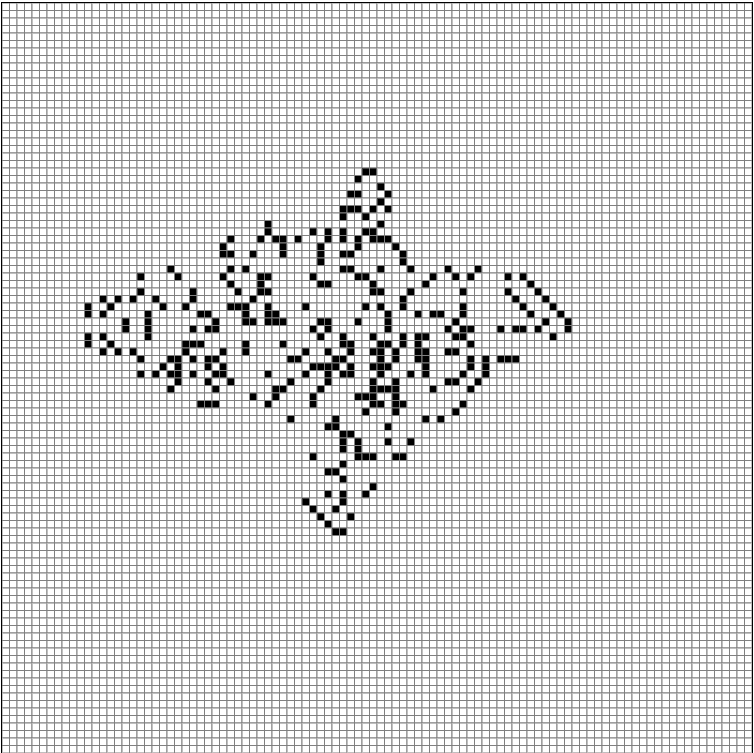
\includegraphics[width=\textwidth]{res/seeds_40.png}
        \subcaption{Krok 40}\label{fig:seeds2}
    \end{minipage}
    \hfill
    \begin{minipage}[t]{.3\textwidth}
        \centering
        
\includegraphics[width=\textwidth]{res/seeds_120.png}
        \subcaption{Krok 120}\label{fig:seeds3}
    \end{minipage}
    \caption{Przykład działania automatu o regule /2 - widoczny znaczny wzrost gęstości żywych komórek (od wartości poniżej 0.01 do około 0.2) pomimo braku warunku na przeżycie komórek.}
    \label{fig:seeds}
\end{figure}

\newpage
Ostatnią regułą poddaną testom w ramach niniejszego dokumentu była reguła \textbf{12345/3}. Wyniki przykładowej symulacji przedstawione zostały na rysunku \ref{fig:lab}. Symulacja przeprowadzona została na sieci o rozmiarach $100\times100$. Gęstość początkowa żywych komórek wyniosła w tym przypadku 0.05. W kolejnych krokach symulacji widocznych na rysunku widoczne jest tworzenie się przypominającej labirynt struktury. Wewnątrz tej struktury stany komórek nie ulegają zmianom. Sytuacja stabilizuje się po zajęciu przez strukturę całej siatki - od tego momentu nie następują już żadne dalsze zmiany. Końcowa gęstość żywych komórek miała wartość 0.54. 

\begin{figure}[H]
    \begin{minipage}[t]{.3\textwidth}
        \centering
        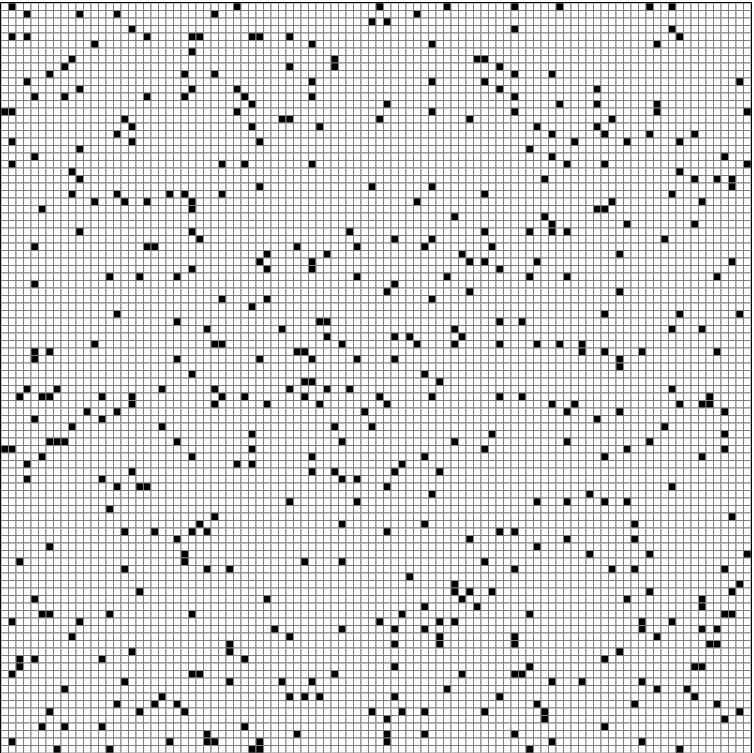
\includegraphics[width=\textwidth]{res/lab_1.png}
        \subcaption{Krok 0}\label{fig:lab1}
    \end{minipage}
    \hfill
    \begin{minipage}[t]{.3\textwidth}
        \centering
        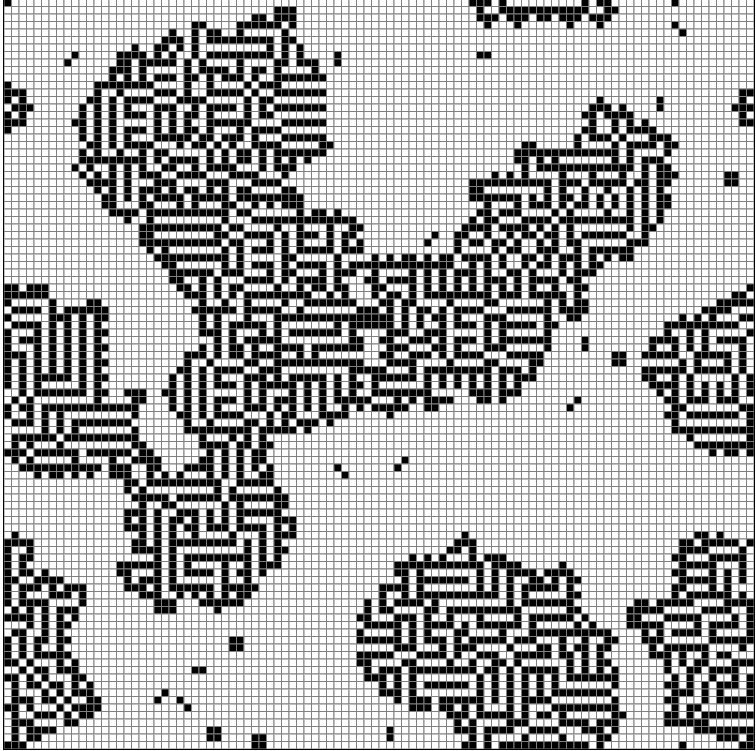
\includegraphics[width=\textwidth]{res/lab_31.png}
        \subcaption{Krok 31}\label{fig:lab2}
    \end{minipage}
    \hfill
    \begin{minipage}[t]{.3\textwidth}
        \centering
        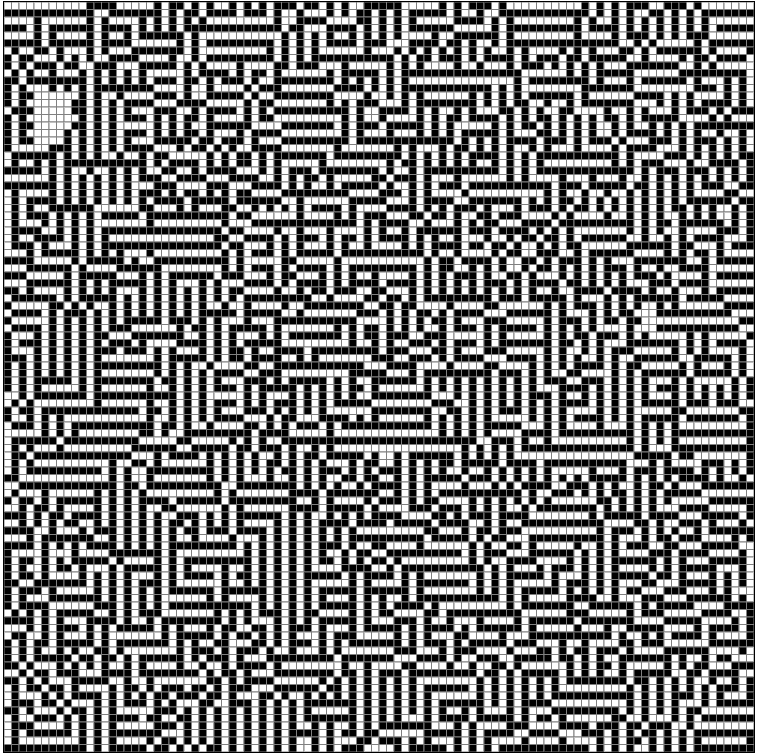
\includegraphics[width=\textwidth]{res/lab_130.png}
        \subcaption{Krok 130}\label{fig:lab3}
    \end{minipage}
    \caption{Przykład działania automatu o regule 12345/3. Widoczne tworzenie się przypominającej labirynt struktury. Rys. \ref{fig:lab3} (krok 130) przedstawia sytuację ustabilizowaną (brak dalszych zmian, gęstość komórek żywych 0.54).}
    \label{fig:lab}
\end{figure}



\section{Wnioski}
\begin{itemize}
\item udało się stworzyć poprawnie działającą implementację dwuwymiarowego automatu komórkowego będącego rozszerzeniem klasycznego automatu \textit{Life}
\item testy przeprowadzone dla klasycznej konfiguracji 23/3 pozwoliły zaobserwować charakterystyczne struktury, takie jak: blok, bochenek, \textit{blinker} czy szybowiec.
\item testy innych konfiguracji pozwoliły zaobserwować charakterystyczne wzorce, takie jak replikator czy labirynt
\item dla klasycznego automatu \textit{Life} testy wykazały, że podanie bardzo niskiej (od około 0 do 0.1) lub bardzo wysokiej (od około 0.8 do 1.0) początkowej gęstości żywych komórek prowadzi do bardzo niskich (nawet zerowych) wartości gęstości w kolejnych krokach czasowych.
\item klasyczny automat \textit{Life} zwykle dąży do stosunkowo niskich wartości wynikowej gęstości.
\item w przypadku reguły 12345/3 utworzenie wzoru labiryntu możliwe jest nawet dla niskich (rzędu 0.03) wartości początkowej gęstości.
\item dla gęstości z przedziału od około 0.2 do 0.7 automat o regule 12345/3 ma tendencje do bardzo szybkiego tworzenia stabilnego labiryntu
\item wzór powstały w wyniku zastosowania reguły /2 ma tendencję do rozprzestrzeniania się po całej sieci
\end{itemize}

\newpage

\begin{thebibliography}{9}

\bibitem{malarz}
  dr hab. inż. Krzysztof Malarz, prof. AGH,
  \emph{wykład prowadzony w ramach przedmiotu Automaty komórkowe},
  \url{http://home.agh.edu.pl/~malarz/dyd/ak/} (dostęp: 17.03.2020)

\bibitem{wiki1}
  Wikipedia, the free encyclopedia,
  \emph{Life-like cellular automaton},
  \url{https://en.wikipedia.org/wiki/Life-like_cellular_automaton} (dostęp: 17.03.2020)

\bibitem{wiki2}
  Wikipedia, the free encyclopedia,
  \emph{Seeds (cellular automaton)},
  \url{https://en.wikipedia.org/wiki/Seeds_(cellular_automaton)} (dostęp: 17.03.2020)

\bibitem{swing}
  Luis Carlos Castillo,
  \emph{Swing Game of Life},
  \url{http://luisccastillo.github.io/Swing-GameOfLife/} (dostęp: 17.03.2020)

\bibitem{d31}
  d3noob,
  \emph{Simple d3.js tooltips},
  \url{https://bl.ocks.org/d3noob/a22c42db65eb00d4e369} (dostęp: 17.03.2020)

\bibitem{d32}
  Yan Holtz,
  \emph{Most basic line chart in d3.js},
  \url{https://www.d3-graph-gallery.com/graph/line_basic.html} (dostęp: 17.03.2020)

\bibitem{bootstrap}
  \emph{Dokumentacja biblioteki Bootstrap w wersji 4.4},
  \url{https://getbootstrap.com/docs/4.4/getting-started/introduction/} (dostęp: 17.03.2020)

\end{thebibliography}

\end{document}